\documentclass[titlepage,a4paper,12pt,AutoFakeBold]{article}
%\NeedsTeXFormat{LaTeX2e}[2005/12/01]
\usepackage{xeCJK}
\setCJKmainfont{SimSun}
%\usepackage[margin=1in]{geometry}
\usepackage{geometry}
\geometry{a4paper,left=3.18cm,right=3.18cm,top=2.54cm,bottom=2.54cm}
\usepackage{braket}
\usepackage{graphicx}


\usepackage[hidelinks]{hyperref}
\hypersetup{
%linkbordercolor={1 1 1},
urlcolor=blue,
}
\usepackage{float}
\usepackage[bottom]{footmisc}

\usepackage{algorithm}
\usepackage[noend]{algpseudocode}
%\usepackage{longtable}
\usepackage{amsmath}
\usepackage{amssymb}
\usepackage{extarrows}
%\usepackage{tabularx}
%\usepackage{rotating}
\usepackage {indentfirst}
\usepackage{courier}
\usepackage[dvipsnames]{xcolor}
\usepackage{listings}
%\usepackage{xcolor}\lstset{}
\lstset{
	basicstyle={\sffamily\footnotesize},
	%	numbers=left,
	%	numberstyle=\tiny\color{gray},
	numbersep=5pt,
	breaklines=true,
	captionpos={T},
	frame={lines},
%%	rulecolor=,
	framerule=0.5pt,
	columns=flexible,
	tabsize=2,
	numbers=left,
%	backgroundcolor = \color{White},
	backgroundcolor={\color{yellow!3!white}}
%	language=Mathematica,
%	keywordstyle=\color{black}
}
\usepackage{enumitem}
%\allowdisplaybreaks[4]
%\usepackage{mathematica}
%\definecolor{darkred}{rgb}{0.5 0 0}
%\definecolor{darkgreen}{rgb}{0.5 .5 0}
%\definecolor{darkblue}{rgb}{0 0 .5}



%\usepackage{listings}
%\renewcommand{\lstlistingname}{Listing}


\renewcommand{\contentsname}{目录}
\newcommand\litem[1]{\item{ #1?\\}}
%\newcommand{\dollar}{\mbox{\textdollar}} \bfseries

\makeatletter

\makeatother






\begin{document}



\title{\textsf{MagneticKP}使用手册}
%\vtitle{利用群表示理论研究三维晶体中的演生粒子}
%\author{张泽英}
\author{张泽英}

\maketitle

%\newpage

\tableofcontents

\newpage

\section{功能简介}
\textsf{MagneticKP}是一款开源的软件包。
该软件包基于线性代数中的迭代算法,可快速构造$k\cdot p$模型。
具体功能如下:
\begin{itemize}
\item   仅需输入对称操作和表示矩阵即可构造出相应的$k\cdot p$模型
\item	可以构造包括磁性、非磁性材料、考虑自旋轨道耦合、大部分自旋群的$k\cdot p$模型
\item	与\textsf{SpaceGroupIrep}(\textsf{MSGCorep})接口后,仅需简单输入空间群(磁群)编号和和不可约表示的编号信息即可构造任意230个空间群(1651个磁群)任意$k$点的$k\cdot p$模型
\item	画能谱图,并且能谱可随参数大小动态显示
\item	读取第一性原理软件的能带结果,拟合参数。
\end{itemize}


\section{安装}

  首先登录github上的\textsf{MagneticKP}程序包首页(无需账号密码):
\begin{center}
\url{https://github.com/zhangzeyingvv/MagneticKP}
\end{center}
点击“Code”,“Download ZIP”,下载MagneticKP-main.zip文件。如下图所示:
\begin{figure}[h]
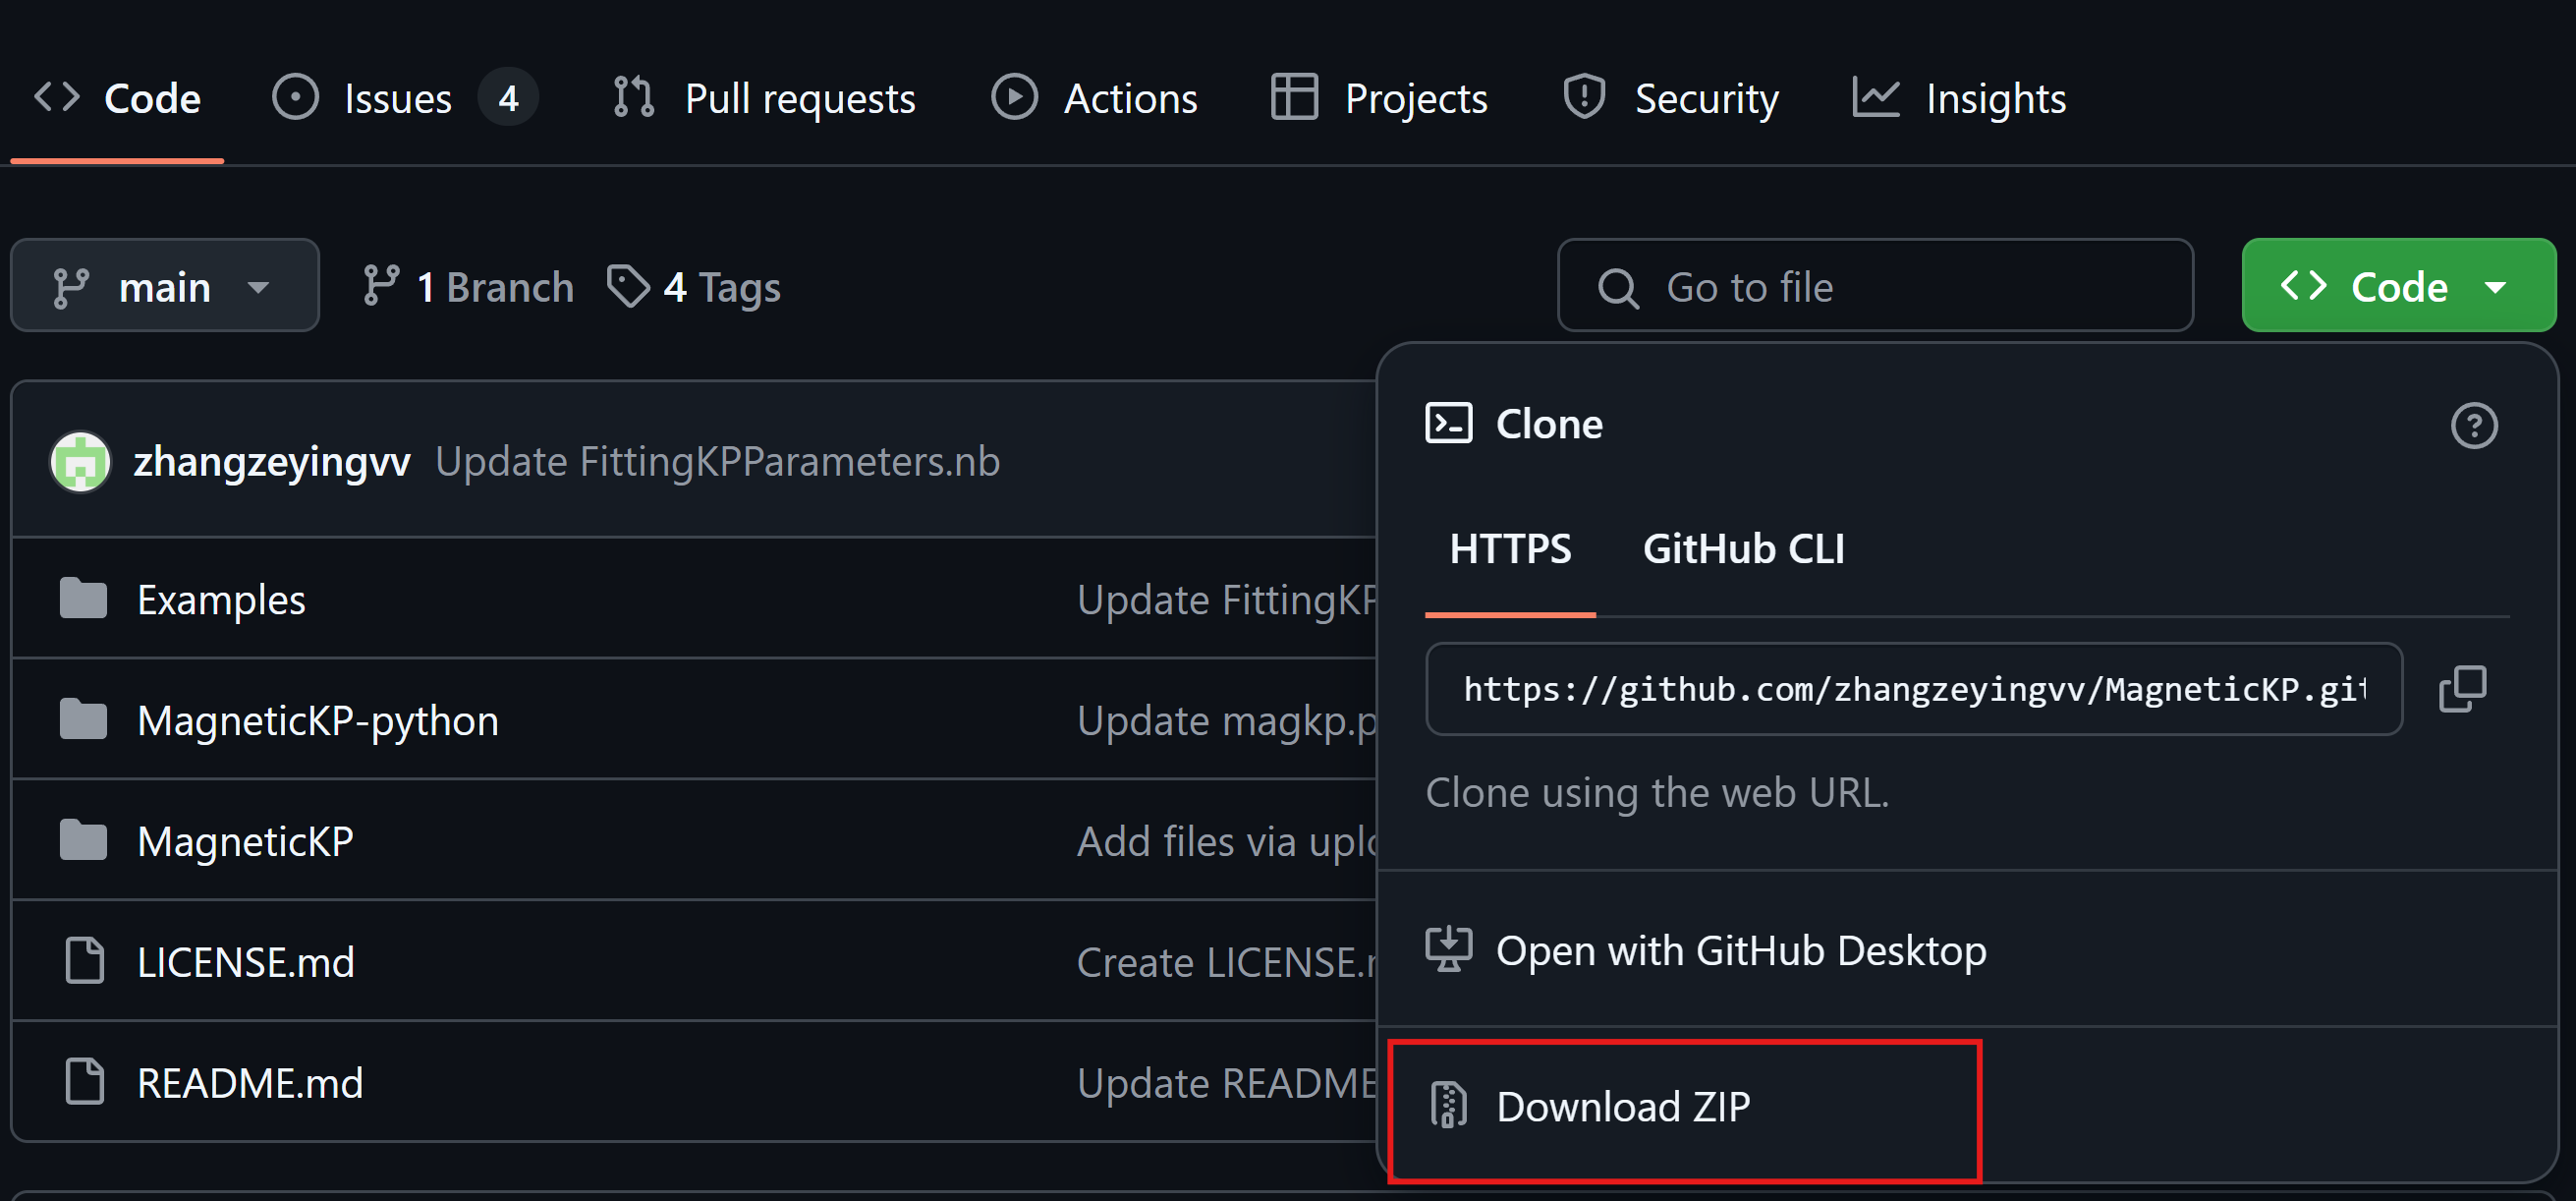
\includegraphics[width=1\textwidth]{./figures/安装1}
\end{figure}


打开Mathematica,运行:
\begin{lstlisting}[numbers=none]
$UserBaseDirectory
\end{lstlisting}
%\lstinline| $\mbox{\$}$ |
运行时点击Shift+回车。打开显示的目录,并进入Applications文件夹。

将刚刚下载的MagneticKP-main.zip解压,会得到一个MagneticKP文件夹和三个文件。把解压得到的MagneticKP文件夹复制到Applications文件夹内,安装完成。在Mathematica中运行
\begin{lstlisting}[numbers=none]
Needs["MagneticKP`"]
\end{lstlisting}	
即可载入程序包。
有经验的用户可以安装到\lstinline|$Path|中任何地方,部分目录需要管理员权限。以上方法对Windows和Linux用户均适用,也可参阅Computer Physics Communications 290, 108784 (2023).


\section{使用方法}
\subsection{核心模块}

\textsf{MagneticKP} 包的核心部分是函数 \lstinline!kpHam!,该函数计算 $\boldsymbol{k}\cdot\boldsymbol{p}$哈密顿量。格式为:
\begin{lstlisting}[backgroundcolor={\color{yellow!5!white}},mathescape=true]
	kpHam[korder, input]
\end{lstlisting}
在这里,\lstinline!korder! 可以是一个整数或一个整数列表,指定要计算的 
$\boldsymbol{k}\cdot\boldsymbol{p}$哈密顿量的截止阶数。当 \lstinline!korder! 是一个列表 
时,\lstinline!kpHam!将输出例表中每个整数 $n$ 对应的哈密顿量的和。当\lstinline!korder! \lstinline!kpHam!将输出阶数小于等于这个整数的哈密顿量\lstinline!input! 的格式为 Mathematica 中的 \lstinline!Association!。它包含构建哈密顿量所需的输入信息。
\lstinline!input!有三个必要的输入:
\begin{itemize}
	\item Q 的旋转部分
	\item Q 的(共)表示矩阵
	\item Q 是幺正算符算符还是反幺正算符
\end{itemize}
\begin{lstlisting}[backgroundcolor={\color{yellow!5!white}},mathescape=true]
	input = <|
	"Unitary" -><|$Q_1$ -> {$D(Q_1)$, $R_1\boldsymbol{k}$},...|>,
	"Anitunitary" -><|$Q_2$ -> {$D(Q_2)$, -$R_2\boldsymbol{k}$},...|>
	|>
\end{lstlisting}
注意,\lstinline|input["Unitary"]| 或 \lstinline|input["Antiunitary"]| 中 \lstinline|Keys| 的作用是使输入更加清晰,\textsf{MagneticKP} 将分别读取 \lstinline|input["Unitary"]| 和 \lstinline|input["Antiunitary"]| 的 \lstinline|Values| 进行计算。
$R_1\boldsymbol{k}$可以使用笛卡尔坐标或分数坐标。用户只需输入 \lstinline|input| 中非空的 \lstinline|Keys|。
当没有反幺正操作时,\lstinline!"Antiunitary"! 不需要作为输入。

\lstinline!kpHam!输出的格式为:
\begin{lstlisting}[backgroundcolor={\color{yellow!5!white}},mathescape=true]
	<|"ham" -> $\boldsymbol{k}\cdot\boldsymbol{p}$ 哈密顿量的表达式,  "korder" -> 哈密顿量的阶数,
	"dim" -> 哈密顿量矩阵的维度, "NumberOfParameters" -> 参数的个数|>
\end{lstlisting}

\subsection{IO 模块}

\lstinline!kpHam!的输入包含小群的表示矩阵 $D(Q_i)$。一般来说,对于 $Q_i\in G$,可以使用投影表示法来获得不可约表示矩阵 $\Delta(Q_i)$计算时比较繁琐。更直接的方法是从教科书或是一些成熟的数据库中获取 $D(Q_i)$。这里,我们给出一个接口函数 \lstinline|interfaceRep| 来与 \textsf{SpaceGroupIrep} 和 \textsf{MSGCorep} 软件包进行接口。

\lstinline|interfaceRep| 的格式为:
\begin{lstlisting}[backgroundcolor={\color{yellow!5!white}},mathescape=true]
	interfaceRep[群编号, k点, 表示的编号, "CartesianCoordinates" -> True or False, "CalculateGenerators" -> True or False]
\end{lstlisting}
其中 \lstinline|MSGNO| 可以是空间群编号(一个整数)或 BNS 磁空间群编号(一个包含两个整数的列表)。当 \lstinline|MSGNO| 是一个整数(列表)时,必须加载 \textsf{SpaceGroupIrep} (\textsf{MSGCorep}) 包。 \lstinline|k| 可以以 $\boldsymbol{K}$坐标形式或 $\boldsymbol{K}$ 点的符号($\boldsymbol{k}$为高对称点)给出。 \lstinline|reps| 是一个整数或整数列表,表示在 \lstinline|showLGIrepTab| (\lstinline|showMLGCorep|) 中不可约(共)表示的序列号。当 \lstinline|reps| 是一个列表时,\textsf{MagneticKP} 将自动计算(共)表示的直和。 \lstinline|"CartesianCoordinates"|(默认值为 \lstinline|True|)告诉 \textsf{MagneticKP} 是否将操作转换为笛卡尔坐标。最后,\lstinline|"CalculateGenerators"|告诉 \textsf{MagneticKP} 是否仅给出小陪群的生成元,若\lstinline|"CalculateGenerators"|为 \lstinline|False| (默认为\lstinline|True|)则输出所有小陪群中的元素。

\subsection{画图模块}

构造出  $\boldsymbol{k}\cdot\boldsymbol{p}$ 模型后将能带画出来或与第一性原理比较可以很直观的检验  $\boldsymbol{k}\cdot\boldsymbol{p}$ 模型的好坏。\textsf{MagneticKP} 提供了三个函数\textsf{bandManipulate,bandplot 和bandManipulateWithVASP}来实现这一点。
\textsf{bandManipulate}可以随参数动态显示 $\boldsymbol{k}\cdot\boldsymbol{p}$ 模型的能带,用法为
\begin{lstlisting}[backgroundcolor={\color{yellow!5!white}},mathescape=true]
	bandManipulate[path, n, ham, "PlotRange" -> {a,b}]
\end{lstlisting}
其中\lstinline|path| 为能带路径,其格式为
\begin{lstlisting}[backgroundcolor={\color{yellow!5!white}},mathescape=true]
	{
		{{$k_1$ 的坐标,$k_2$ 的坐标 },{$k_1$,$k_2$}},
		{{$k_3$ 的坐标,$k_4$ 的坐标},{$k_3$,$k_4$}},
		$\cdots$
	};\end{lstlisting}
\lstinline|n| 为每段能带的撒点数,\lstinline|ham|为 \lstinline|kpHam| 输出的哈密顿量,\lstinline|"PlotRange"| 为能带的能量范围。
\lstinline|bandplot| 可以用来画标好高对称点的能带图,其用法为
\begin{lstlisting}[backgroundcolor={\color{yellow!5!white}},mathescape=true]
bandplot[path,n,ham,rule ,"PlotRange"->{a,b}]
\end{lstlisting}
其中\lstinline|path| 为能带路径,\lstinline|n| 为每段能带的撒点数,\lstinline|ham|为 \lstinline|kpHam| 输出的哈密顿量,\lstinline|rule| 为哈密顿量中参数的大小,\lstinline|"PlotRange"| 为能带的能量范围。
\lstinline|bandManipulateWithVASP| 可以同时显示第一性原理和  $\boldsymbol{k}\cdot\boldsymbol{p}$ 模型的能带用法详见 ``FittingKPParameters.nb" 文件

\section{例子}
计算13号空间群($P2/c$) $\ensuremath{B(-\frac{1}{2},0,0)}$ 点 $B_{2}$ 不可约表示对应的 $k\cdot p$ 模型.
$B$ 点小陪群的生成元可以选择为 $C_{2z}$ 和 $I$ . 那么 $Rk$ 及 $B_{2}$ 表示矩阵可以写为
\begin{align*}
	C_{2z} & :(k_{x},k_{y},k_{z})\rightarrow(-k_{x},-k_{y},k_{z})\\
	I & :(k_{x},k_{y},k_{z})\rightarrow(-k_{x},-k_{y},-k_{z})\\
	D(C_{2z}) & =\sigma_{1},D(I)=\sigma_{3}
\end{align*}
因此,仅需输入
\begin{lstlisting}[backgroundcolor={\color{yellow!5!white}},mathescape=true]
	Needs["MagneticKP`"];
	input =<|"Unitary" -> <|C2z -> {{{0, 1}, {-1, 0}}, {-kx, -ky, kz}}, I -> {{{1, 0}, {0, -1}}, {-kx, -ky, -kz}}|>|>;
	kpHam[1, input]["ham"]
\end{lstlisting}
若不想自己计算表示矩阵,仅需与\textsf{MSGCorep}软件包接口。首先看一下$P2/c$ $\ensuremath{B(-\frac{1}{2},0,0)}$有哪些不可约表示
\begin{lstlisting}[backgroundcolor={\color{yellow!5!white}},mathescape=true]
	Needs["MSGCorep`"];
	showMLGCorep[{13, 65}, "B"]
\end{lstlisting}
结果为
\begin{figure}[H]
	\centering
	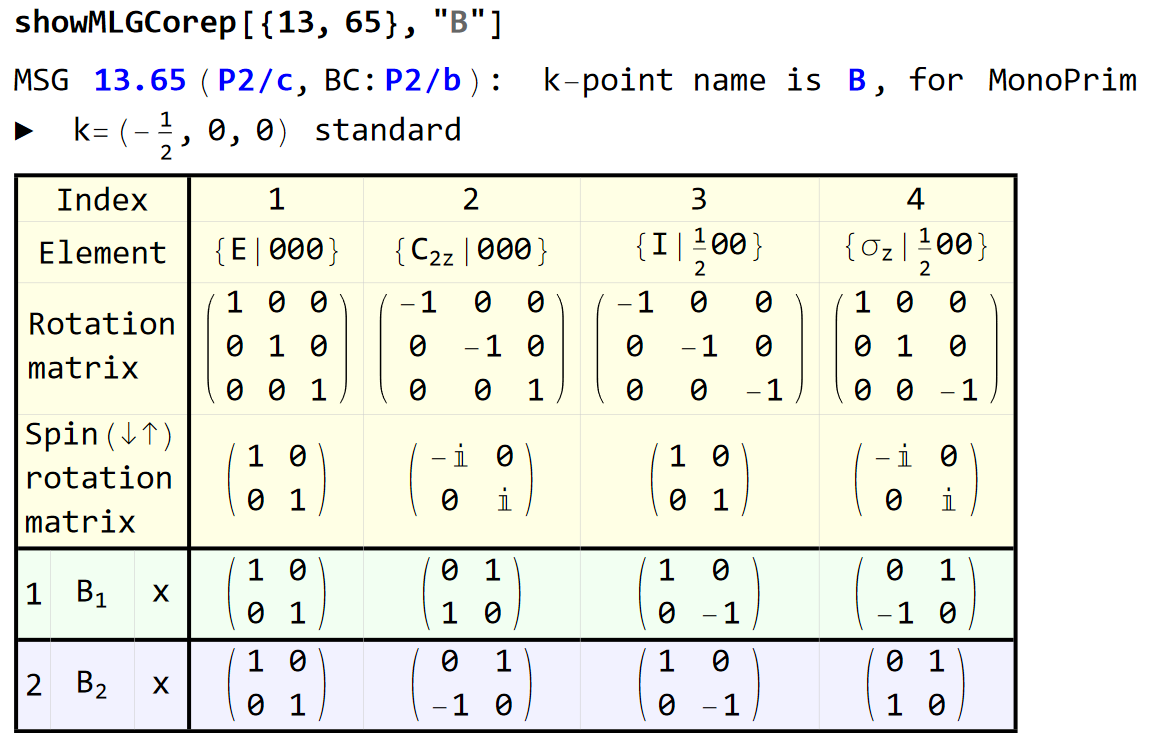
\includegraphics[width=.5\textwidth]{./figures/showcorep}
\end{figure}
可以看到 $B_2$ 对应\lstinline|showMLGCorep|的第二个表示,用\lstinline|interfaceRep|获取表示矩阵
\begin{lstlisting}[backgroundcolor={\color{yellow!5!white}},mathescape=true];
	input = interfaceRep[{13, 65}, "B", {2}]
	ham=kpHam[1, input]["ham"]
\end{lstlisting}
得到的哈密顿量与手动输入完全相同为:
\[
H(\boldsymbol{k})=\varepsilon+c_{1}\sigma_{1}k_{x}+c_{2}\sigma_{1}k_{y}+c_{3}\sigma_{2}k_{z}
\]
可以利用 \lstinline|bandManipulate| 动态显示能带
\begin{lstlisting}[backgroundcolor={\color{yellow!5!white}},mathescape=true]
	path = {{{{1/3, 0, 0}, {0, 0, 0}}, {"X", "B"}},
		{{{0, 0, 0}, {0, 1/3, 0}}, {"B", "Y"}},
		{{{0, 0, 0}, {0, 0, 1/3}}, {"B", "Z"}}
	};
	bandManipulate[path, 100, ham, 
	"PlotRange" -> {-2, 2}]
\end{lstlisting}
结果为
\begin{figure}[H]
	\centering
	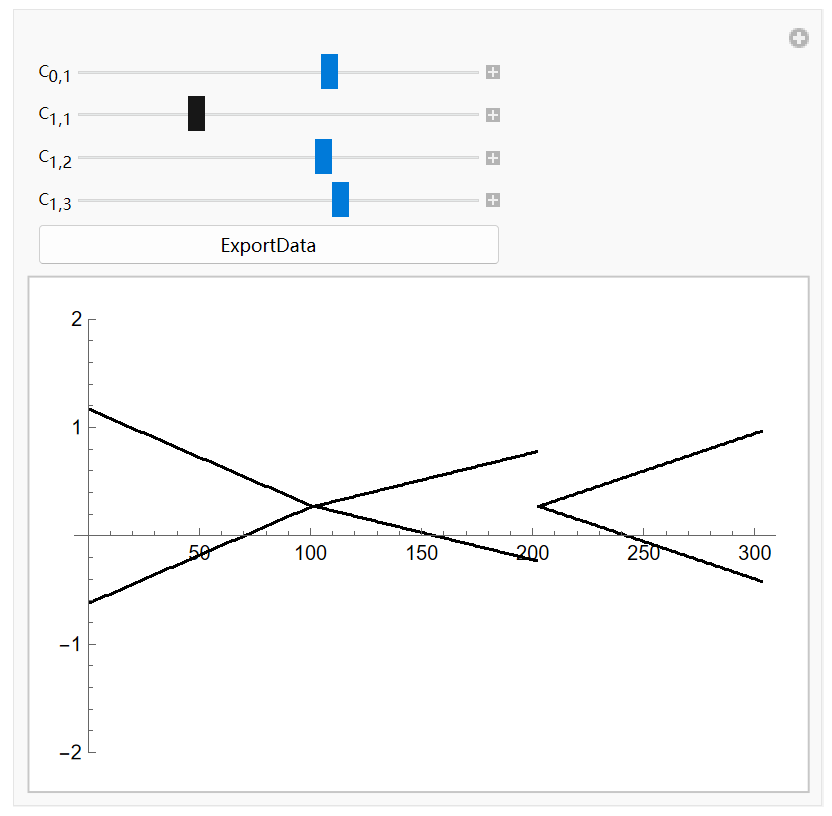
\includegraphics[width=.5\textwidth]{./figures/bandm}
\end{figure}
确定好参数后,可以用\lstinline|bandplot|画出比较好看的能带图
\begin{lstlisting}[backgroundcolor={\color{yellow!5!white}},mathescape=true]
bandplot[path,200,ham,{$C_{0,1}$->0.27,$C_{1,1}$->-0.425,$C_{1,2}$->0.24,$C_{1,3}$->0.33},"PlotRange"->{-1,1}]
\end{lstlisting}
结果为
\begin{figure}[H]
	\centering
	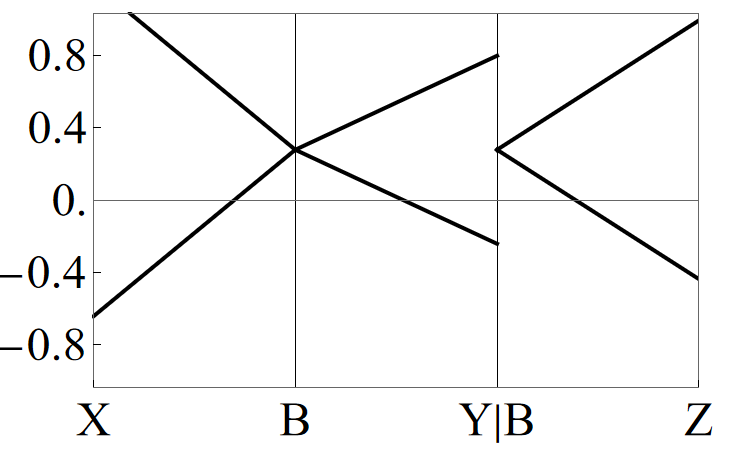
\includegraphics[width=.5\textwidth]{./figures/band}
\end{figure}
更多例子请参阅example.nb文件。
\section{常见问题}
    \begin{enumerate}[style=nextline]
    \setlength\itemsep{1.5em}
	\litem{安装完以后运行没反应怎么办} 
	
	回答:仔细检查安装步骤,先把examples.nb文件中几个例子跑出来,实在不行在QQ群里提问。

	\litem{QQ群怎么加} 
	回答:群号为625192239。可以扫描以下二维码:

\begin{figure}[H]
	\centering
	
\includegraphics[width=.3\textwidth]{./figures/QQ}
\end{figure}

	\litem{想构造非磁材料的$k\cdot p$ 模型,应该和\textsf{SpaceGroupIrep}接口吗?} 
	
	回答:一般非磁材料均有时间反演对称性,用于描述具有时间反演对称性的群为第二类磁群,即灰群。而\textsf{SpaceGroupIrep}虽然给出了每一个不可约表示表示的类型,但没有给出共表示矩阵。因此要计算第二类磁群的 $k\cdot p$ 模型还是需要和\textsf{MSGCorep}接口。
	
	\litem{我发现了Bug,该怎么办}
	
	回答:在\url{https://github.com/zhangzeyingvv/MagneticKP/issues}上提问,在QQ群里提问,给我发邮件zhangzeyingvv@gmail.com。
		
	
	\litem{\textsf{MagneticKP}支持构造自旋群的$k\cdot p$模型吗}

	回答:只要给出表示矩阵和对称操作,\textsf{MagneticKP}就可以给出$k\cdot p$模型。但是自旋群表示矩阵需要自己计算。
		
	\litem{可以转发该手册吗}

	回答:可以转发,同时如果想修改本手册,请通过github向我提issue(s)。

	\litem{如何引用\textsf{MagneticKP}}

    回答:Zeying Zhang, Zhi-Ming Yu, Gui-Bin Liu, Zhenye Li, Shengyuan A. Yang, Yugui Yao,
    Computer Physics Communications, 290, 108784 (2023)
    
    BibTeX:
    \begin{lstlisting}[numbers=none,language=TeX]
    	@article{ZHANG2023108784,
    		title = {MagneticKP: A package for quickly constructing k⋅p models of magnetic and non-magnetic crystals},
    		journal = {Computer Physics Communications},
    		volume = {290},
    		pages = {108784},
    		year = {2023},
    		issn = {0010-4655},
    		doi = {https://doi.org/10.1016/j.cpc.2023.108784},
    		url = {https://www.sciencedirect.com/science/article/pii/S0010465523001297},
    		author = {Zeying Zhang and Zhi-Ming Yu and Gui-Bin Liu and Zhenye Li and Shengyuan A. Yang and Yugui Yao}
    	}
    \end{lstlisting}
\end{enumerate}



\end{document}
